\documentclass[tikz,border=3mm]{standalone}
\usepackage{amsmath}
\usetikzlibrary{arrows.meta,calc,positioning}

\begin{document}
\pagecolor{white}
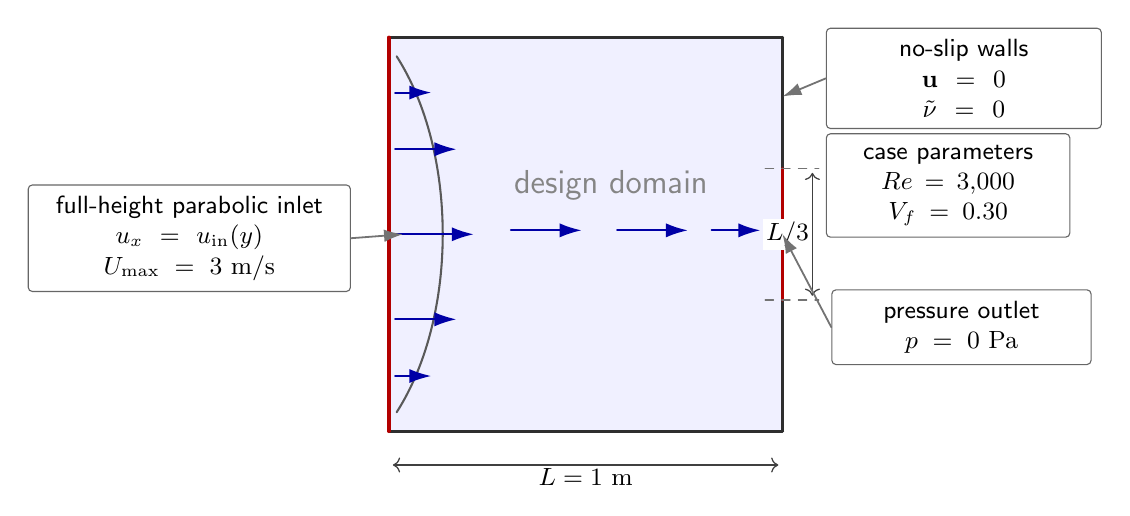
\begin{tikzpicture}[
  line cap=round,
  line join=round,
  font=\sffamily\small,
  flow/.style={-{Latex[length=2.8mm,width=1.8mm]}, line width=0.75pt, draw=blue!65!black},
  dim/.style={<->, line width=0.45pt, draw=black!75, shorten <=1.5pt, shorten >=1.5pt},
  bc/.style={draw=black!60, fill=white, rounded corners=1.5pt, inner xsep=7pt, inner ysep=4pt, align=center},
  wall/.style={draw=black!82, line width=1.1pt},
  boundary/.style={draw=red!70!black, line width=1.35pt},
  profile/.style={draw=black!65, line width=0.75pt},
  guide/.style={draw=black!55, dashed, line width=0.45pt},
  dimlabel/.style={fill=white, inner sep=1pt, font=\sffamily\small},
  designlabel/.style={font=\sffamily\large, text=black!48}
]

\def\L{5.0}
\def\outLow{1.6667}
\def\outHigh{3.3333}
\def\outMid{2.5}

% Design domain.
\fill[blue!6] (0,0) rectangle (\L,\L);
\node[designlabel] at (2.82,3.12) {design domain};

% No-slip wall segments.
\draw[wall] (0,\L) -- (\L,\L);
\draw[wall] (0,0) -- (\L,0);
\draw[wall] (\L,0) -- (\L,\outLow);
\draw[wall] (\L,\outHigh) -- (\L,\L);

% Boundary sections.
\draw[boundary] (0,0) -- (0,\L);
\draw[boundary] (\L,\outLow) -- (\L,\outHigh);

% Parabolic inlet velocity profile and representative vectors.
\draw[profile]
  (0.10,0.24) .. controls (0.88,1.46) and (0.88,3.54) .. (0.10,4.76);
\foreach \y/\xend in {0.70/0.54,1.42/0.86,2.50/1.08,3.58/0.86,4.30/0.54}{
  \draw[flow] (0.08,\y) -- (\xend,\y);
}

% Interior flow indication.
\draw[flow] (1.55,2.55) -- (2.45,2.55);
\draw[flow] (2.90,2.55) -- (3.80,2.55);
\draw[flow] (4.10,2.55) -- (4.72,2.55);

% Outlet and domain dimensions.
\draw[guide] (4.78,\outLow) -- (5.46,\outLow);
\draw[guide] (4.78,\outHigh) -- (5.46,\outHigh);
\draw[dim] (5.38,\outLow) -- node[dimlabel, left] {$L/3$} (5.38,\outHigh);
\draw[dim] (0,-0.43) -- node[dimlabel, below] {$L=1~\mathrm{m}$} (\L,-0.43);

% Boundary-condition labels.
\node[bc, anchor=east, text width=36mm] (inletLabel) at (-0.48,2.45)
  {full-height parabolic inlet\\$u_x=u_{\mathrm{in}}(y)$\\$U_{\max}=3~\mathrm{m/s}$};
\draw[-{Latex[length=2.4mm,width=1.6mm]}, black!55, line width=0.65pt]
  (inletLabel.east) -- (0.18,2.50);

\node[bc, anchor=west, text width=28mm] (outletLabel) at (5.62,1.32)
  {pressure outlet\\$p=0~\mathrm{Pa}$};
\draw[-{Latex[length=2.4mm,width=1.6mm]}, black!55, line width=0.65pt]
  (outletLabel.west) -- (5.00,\outMid);

\node[bc, anchor=west, text width=30mm] (wallLabel) at (5.55,4.48)
  {no-slip walls\\$\mathbf{u}=0$\\$\tilde{\nu}=0$};
\draw[-{Latex[length=2.4mm,width=1.6mm]}, black!55, line width=0.65pt]
  (wallLabel.west) -- (5.00,4.25);

\node[bc, anchor=west, text width=26mm] at (5.55,3.12)
  {case parameters\\$Re=3{,}000$\\$V_f=0.30$};

\end{tikzpicture}
\end{document}
